\vspace*{0.3cm} \noindent
\subsubsection{Desarrollo Implementacion C}

En esta implementación, inicialmente,se crearon dos punteros de matriz uno correspondiente a src y otro a dst.\newline 
Ademas, un entero llamado $suma$ y otro $divido$ inicializados en 0. \newline
Luego, realizamos dos ciclos, uno añidado dentro del otro recorriendo de la forma $'(int\ i\_d = 0;\ i\_d < filas;\ i\_d++)'$ y 
$(int\ j\_d = 0;\ j\_d < cols;\ j\_d++)$.\newline
Dentro del segundo ciclo, creamos dos punteros rgb\_t donde uno apuntará a \newline rgb\_t $*p\_d = (rgb\_t*)\  \&dst\_matrix[i\_d][j\_d*3]$, y el otro
a $rgb\_t *p\_s = (rgb\_t*)\ \&src\_matrix[i\_d][j\_d]$.\newline
Al entero $suma$ le guardamos la suma de los correspondientes r, g y b del puntero p\_s $suma = p\_s\rightarrow r + p\_s\rightarrow b + p\_s\rightarrow g$
Al entero $divido$ le guardamos el valor de suma dividido por 3 $ divido = suma/3$
Posteriormente, chequeamos entre que valores se encuentra divido utilizando la funcion between provista por la catedra:\vspace*{0.3cm} \noindent\newline 
Primero si $(between(divido,0,31))$, en caso verdadero, guardamos en el valor r del puntero p\_d el valor 0,en el valor g 
guardamos el valor 0 y en el valor b guardamos $(128+ (4*divido)$. \newline 
Segundo, si $(between(divido,32,95))$, en caso verdadero, guardamos en el valor r del puntero p\_d el valor 0,en el valor g 
guardamos el valor $(divido-32)*4$ y en el valor b guardamos 255. \newline Tercero, si $(between(divido,96,159))$, en caso verdadero, guardamos en el valor r del puntero p\_d el valor $(divido-96)*4$,en el valor g 
guardamos el valor 255 y en el valor b guardamos $255-((divido-96)*4)$. \newline Cuarto, si $(between(divido,160,223))$, en caso verdadero, guardamos en el valor r del puntero p\_d el valor 255,en el valor g 
guardamos el valor $255 - ((divido-160)*4)$ y en el valor b guardamos 0. \newline  Por ultimo, si $(between(divido,224,255))$, en caso verdadero, guardamos en el valor r del puntero p\_d el valor $255-(divido-224)*4$,en el valor g 
guardamos el valor 0 y en el valor b guardamos 0. \newline 

Estos dos ciclos realizaran $j\_d = cols - 1$  por $i\_d = filas -1$ de itereaciones.\newline
Con lo mencionado, obtenemos el filtro temperature en c correctamente, con los valores que nos pasan como parámetros.\newline

\vspace*{0.3cm} \noindent
\subsubsection{Desarrollo Implementacion en ASM}
En esta implementacion, inicialmente pusheamos RBP, R12 y R13, nos guardamos en R12 y R13 los respectivos valores de columnas y filas.\newline
Luego, guardamos en EAX un 3, guardamos en R10D, R13D y procedemos a hacer la operacion MUL R10, luego realizamos lo mismo con R12 y así,
obtenemos en R10 el valor completo de la cantidad de pixeles a recorrer.\newline
Guardamos en R11 el valor de RDI donde venia *src y en R13 el valor de RSI donde venia *dst. \newline
Luego, realizamos la seccion donde chequeamos si estamos en el final de la linea o mejor dicho en el padding, comparamos con R10D si es cero \newline
en caso de ser 0 significa que ya recorrimos toda la imagen completa por ende saltamos a la etiqueta fin. \newline
En caso de no ser cero, comparamos r15d con 15, en r15 teníamos guardado la cantidad de pixel que vamos a recorrer en una iteracion.
Como vemos de a 15 pixeles si el valor es menor significa que estamos por tocar el padding y eso lo chequeamos a parte. \newline
Si no es menor, procedemos a recorrer y trabajar con 15 pixeles de la siguiente forma: \newline
Primero, nos guardamos en XMM0 los primeros 15 pixeles haciendo $ movdqu\  XMM0, [RDI]$, luego, el valor de XMM0,
lo guardamos en XMM1 y XMM2, limpiamos XMM7 y con 3 mascaras distintas que lo que hacen es ponernos los 5 pixeles rojos adelante y llenar con 0, 
los 5 pixeles azules y llenar con cero y los 5 pixeles verdes y llenar con ceros. \newline
Realizamos la operacion Pshufb con los tres xmm y las mascaras (un xmm con cada mascara) y luego desempaquetamos de byte a word,
usando el xmm7 que habiamos llenado de 0. \newline
El desempaquetado hace que nos queden los valores en word en los registros XMM10, XMM12, XMM14 respectivamente, y luego
los sumamos con PADDW guardando el valor en XMM10. De esta forma obtenemos en word 
$|b0 + g0 + r0|b1 + g1 + r1|b2 + g2 + r2|b3 + g3 + r3|b4 + g4 + r4|$. \newline
Limpiamos todos los registros que usamos, salvo XMM10 y volvemos a guardar en XMM0 el valor de XMM10. Luego, procedemos
a realizar la division correspondiente de los packs de la siguiente manera:\newline

$movdqu xmm10, [DIVIDO]$\newline$
$\hspace*{2.3cm}$	movdqu xmm1, xmm0$\newline$
$\hspace*{2.8cm}$		movdqu xmm2, xmm0$\newline$
		$\hspace*{2.8cm}$XORPD xmm15, xmm15$\newline$
		$\hspace*{2.8cm}$punpcklwd xmm1, xmm15$\newline$
		$\hspace*{2.8cm}$punpckhwd xmm2, xmm15$\newline$
		$\hspace*{2.8cm}$cvtdq2ps xmm1, xmm1$\newline$
		$\hspace*{2.8cm}$cvtdq2ps xmm2, xmm2$\newline$
		$\hspace*{2.8cm}$cvtdq2ps xmm10,xmm10$\newline$
		$\hspace*{2.8cm}$divps XMM1, xmm10$\newline$
		$\hspace*{2.8cm}$divps XMM2, xmm10$\newline$
		$\hspace*{2.8cm}$CVTTPS2DQ xmm1,xmm1$\newline$
		$\hspace*{2.8cm}$CVTTPS2DQ xmm2, xmm2$\newline$
		$\hspace*{2.8cm}$PACKUSDW xmm1, xmm2$\newline$
		$\hspace*{2.8cm}$movdqu xmm0, xmm1$\newline$
		 $$\newline$
	
En la mascara DIVIDO tenemos el valor 3 en DD. Desempaquetamos de Word a Dword para luego podes convertir a float.
Realizamos la respectiva division y luego volvemos a convertir de float a dword y de dword a word y volvemos a guardar
el resultado en XMM0. \newline

Limpiamos todos los registros que usamos, salvo XMM0. Posteriormente, seguimos con las comparaciones.
Primero, vamos a comparar si nuestras sumas son mayores a 223, guardamos en XMM14 el valor 223 con una mascara en DW la cual tiene en todos los pack
el 223. Guardamos en XMM15 el valor XMM0 y comparamos con XMM14.
A partir del resultado en XMM15 realizamos lo siguiente:\newline

$\hspace*{2.3cm}$$movdqu\ xmm13,\ xmm0$\newline$
		$\hspace*{2.8cm}$movdqu\ xmm11, [M224]$\newline$		
		$\hspace*{2.8cm}$psubb\ XMM13,\ xmm11$\newline$
		$\hspace*{2.8cm}$pand\ xmm13,\ xmm15$\newline$
			$\hspace*{2.8cm}$movdqu\ xmm11, [M4]$\newline$
		$\hspace*{2.8cm}$movdqu\ xmm7,\ xmm13$\newline$
		$\hspace*{2.8cm}$movdqu\ xmm8,\ xmm13$\newline$
		$\hspace*{2.8cm}$XORPD\ xmm9,\ xmm9$\newline$
		$\hspace*{2.8cm}$punpcklwd\ xmm7,\ xmm9$\newline$
		$\hspace*{2.8cm}$punpckhwd\ xmm8,\ xmm9$\newline$
		$\hspace*{2.8cm}$cvtdq2ps\ xmm7,\ xmm7$\newline$
		$\hspace*{2.8cm}$cvtdq2ps\ xmm8,\ xmm8$\newline$
		$\hspace*{2.8cm}$cvtdq2ps\ xmm11,xmm11$\newline$
		$\hspace*{2.8cm}$mulps\ XMM7,\ xmm11$\newline$
		$\hspace*{2.8cm}$mulps\ XMM8,\ xmm11$\newline$
		$\hspace*{2.8cm}$CVTPS2DQ\ xmm7,xmm7$\newline$
		$\hspace*{2.8cm}$CVTPS2DQ\ xmm8,\ xmm8$\newline$
		$\hspace*{2.8cm}$PACKUSDW\ xmm7,\ xmm8$\newline$
		$\hspace*{2.8cm}$movdqu\ xmm13,\ xmm7$\newline$
		$\hspace*{2.8cm}$movdqu\ xmm11, [M255]$\newline$
		$\hspace*{2.8cm}$pand\ xmm11,\ xmm15$\newline$
		$\hspace*{2.8cm}$psubb\ xmm11,\ xmm13$\newline$
		$\hspace*{2.8cm}$movdqu\ xmm13,\ xmm11$\newline$		
		$\hspace*{2.8cm}$pshufb\ xmm13, [MASK_5] $\newline$
		$\hspace*{2.8cm}$PADDUSW\ XMM10,\ XMM15 $\newline$
		$\hspace*{2.8cm}$movdqu\ xmm11,\ xmm15 $\newline$
		$\hspace*{2.8cm}$pcmpeqw\ XMM14,XMM14$\newline$
		$\hspace*{2.8cm}$pxor\ xmm11,\ xmm14$\newline$
		$\hspace*{2.8cm}$pand\ xmm0,xmm11$\newline$		
		$\hspace*{2.8cm}$pshufb\ XMM15, [MASK_DE1WORDA3BYTES]$\newline$
		$\hspace*{2.8cm}$pand\ xmm13,\ xmm15$\newline$
		$\hspace*{2.8cm}$movdqu\ xmm5,\ xmm13$$\newline$

Copiamos en XMM13, el valor de XMM0, guardamos en XMM11 una mascara en DW con 224, realizamos la resta de los packs y luego un and 
con XMM15 para quedarnos con los packs que cumplieron esta comparacion. Despues, guardamos en XMM11 una mascara en DW con 4.
Procedemos a desempaquetar de WORD a DWORD el XMM13 copiandolo previamente en otros dos XMM. Luego convertimos todo de DWORD
a FLOAT y realizamos la multiplicacion con XMM11. Volvemos a convertir a DWORD y a empaquetar a WORD y guardamos el resultado 
en XMM13. \newline
Guardamos en XMM11 una mascara DW con 255 realizamos un and entre este XMM y el XMM15 para quedarnos con los packs que dieron TRUE
la comparacion y luego restamos XMM11 con XMM13 y guardamos el valor de XMM11 en XMM13.
En MASK\_5 tenemos en DW los pack de los resultados que da el caso 5 osea $X|0|0$. Luego, en\ XMM10 lo usamos para saturar en 1 los casos que ya 
son chequeados para así no pisarlos con los otros casos. \newline
Lo salvamos y lo invertimos osea de 00 a FF y viceversa y luego hacemos un AND con los pack de\ XMM0 para quedarnos con los valores que no dieron TRUE. \newline
Usamos una mascara para que nos acomode todo de 1word a 3 bytes, hacemos otro AND con los valores TRUE y lo guardamos en\ XMM5. \newline

Despues de chequear este caso pasamos al caso 4: \newline

Primero, vamos a comparar si nuestras sumas son mayores a 159, guardamos en XMM14 el valor 159 con una mascara en DW la cual tiene en todos los pack
el 159. Guardamos en XMM15 el valor XMM0 y comparamos con XMM14.
A partir del resultado en XMM15 realizamos lo siguiente: \newline

$\hspace*{2.3cm}$$movdqu\ xmm13,\ xmm0$\newline$
		$\hspace*{2.8cm}$movdqu\ xmm11, [M160]$\newline$	
		$\hspace*{2.8cm}$psubb\ XMM13,\ xmm11$\newline$
		$\hspace*{2.8cm}$pand\ xmm13,\ xmm15$\newline$
		$\hspace*{2.8cm}$movdqu\ xmm11, [M4]$\newline$
		$\hspace*{2.8cm}$movdqu\ xmm7,\ xmm13$\newline$
		$\hspace*{2.8cm}$movdqu\ xmm8,\ xmm13$\newline$
		$\hspace*{2.8cm}$XORPD\ xmm9,\ xmm9$\newline$
		$\hspace*{2.8cm}$punpcklwd\ xmm7,\ xmm9$\newline$
		$\hspace*{2.8cm}$punpckhwd\ xmm8,\ xmm9$\newline$
		$\hspace*{2.8cm}$cvtdq2ps\ xmm7,\ xmm7$\newline$
		$\hspace*{2.8cm}$cvtdq2ps\ xmm8,\ xmm8$\newline$
		$\hspace*{2.8cm}$cvtdq2ps\ xmm11,xmm11$\newline$
		$\hspace*{2.8cm}$mulps\ XMM7,\ xmm11$\newline$
		$\hspace*{2.8cm}$mulps\ XMM8,\ xmm11$\newline$
		$\hspace*{2.8cm}$CVTPS2DQ\ xmm7,xmm7$\newline$
		$\hspace*{2.8cm}$CVTPS2DQ\ xmm8,\ xmm8$\newline$
		$\hspace*{2.8cm}$PACKUSDW\ xmm7,\ xmm8$\newline$
		$\hspace*{2.8cm}$movdqu\ xmm13,\ xmm7
		$\newline$
		$\hspace*{2.8cm}$movdqu\ xmm11, [MASK\_4]$\newline$
		$\hspace*{2.8cm}$pshufb\ xmm13, [MASK\_4\_2]$\newline$
		$\hspace*{2.8cm}$psubb\ xmm11,\ xmm13 $\newline$
		$\hspace*{2.8cm}$movdqu\ xmm13,\ xmm11$\newline$
		$\hspace*{2.8cm}$movdqu\ xmm11,\ xmm15$\newline$
		$\hspace*{2.8cm}$pcmpeqw\ XMM14,XMM14$\newline$
		$\hspace*{2.8cm}$pxor\ xmm11,\ xmm14$\newline$
		$\hspace*{2.8cm}$pand\ xmm0,xmm11$\newline$
		$\hspace*{2.8cm}$PADDUSW\ XMM10,\ XMM15 $\newline$
		$\hspace*{2.8cm}$pshufb\ XMM15, [MASK\_DE1WORDA3BYTES]$\newline$
		$\hspace*{2.8cm}$pand\ xmm13,\ xmm15$\newline$
		$\hspace*{2.8cm}$movdqu\ xmm4,\ xmm13$$\newline$

		

Copiamos en XMM13, el valor de XMM0, guardamos en XMM11 una mascara en DW con 160, realizamos la resta de los packs y luego un and 
con XMM15 para quedarnos con los packs que cumplieron esta comparacion. Despues, guardamos en XMM11 una mascara en DW con 4.
Procedemos a desempaquetar de WORD a DWORD el XMM13 copiandolo previamente en otros dos XMM. Luego convertimos todo de DWORD
a FLOAT y realizamos la multiplicacion con XMM11. Volvemos a convertir a DWORD y a empaquetar a WORD y guardamos el resultado 
en XMM13. \newline
Guardamos en XMM11 una mascara DW con los resultados que da el caso 4 y hacemos un movimiento de Packs en XMM13 de la forma
$X|0x80|0x80$ realizamos la resta entre ambos y guardamos el resultado de XMM11 en XMM13. Guardamos en XMM11 el valor de XMM15 
invertimos el XMM11 y luego hacemos un and con XMM0.\newline
Luego, en\ XMM10 lo usamos para saturar en 1 los casos que ya son chequeados para así no pisarlos con los otros casos. \newline
Usamos una mascara para que nos acomode todo de 1word a 3 bytes, hacemos otro AND con los valores TRUE y lo guardamos en\ XMM4. \newline

Despues de chequear este caso pasamos al caso 3: \newline

Primero, vamos a comparar si nuestras sumas son mayores a 95, guardamos en\ XMM14 el valor 95 con una mascara en DW la cual tiene en todos los pack
el 95. Guardamos en\ XMM15 el valor\ XMM0 y comparamos con\ XMM14.
A partir del resultado en\ XMM15 realizamos lo siguiente:\newline

	$\hspace*{2.3cm}$$movdqu\ xmm13,\ xmm0$\newline$
		$\hspace*{2.8cm}$movdqu\ xmm11, [M96]$\newline$	
		$\hspace*{2.8cm}$psubb\ XMM13,\ XMM11$\newline$
		$\hspace*{2.8cm}$pand\ xmm13,\ xmm15$\newline$
		$\hspace*{2.8cm}$movdqu\ xmm11, [M4]$\newline$
		$\hspace*{2.8cm}$movdqu\ xmm7,\ xmm13$\newline$
		$\hspace*{2.8cm}$movdqu\ xmm8,\ xmm13$\newline$
		$\hspace*{2.8cm}$XORPD\ xmm9,\ xmm9$\newline$
		$\hspace*{2.8cm}$punpcklwd\ xmm7,\ xmm9$\newline$
		$\hspace*{2.8cm}$punpckhwd\ xmm8,\ xmm9$\newline$
		$\hspace*{2.8cm}$cvtdq2ps\ xmm7,\ xmm7$\newline$
		$\hspace*{2.8cm}$cvtdq2ps\ xmm8,\ xmm8$\newline$
		$\hspace*{2.8cm}$cvtdq2ps\ xmm11,xmm11$\newline$
		$\hspace*{2.8cm}$mulps\ XMM7,\ xmm11$\newline$
		$\hspace*{2.8cm}$mulps\ XMM8,\ xmm11$\newline$
		$\hspace*{2.8cm}$CVTPS2DQ\ xmm7,xmm7$\newline$
		$\hspace*{2.8cm}$CVTPS2DQ\ xmm8,\ xmm8$\newline$
		$\hspace*{2.8cm}$PACKUSDW\ xmm7,\ xmm8$\newline$
		$\hspace*{2.8cm}$movdqu\ xmm13,\ xmm7$\newline$
		$\hspace*{2.8cm}$pshufb\ xmm13, [MASK\_3] $\newline$
		$\hspace*{2.8cm}$movdqu\ xmm11, [MASK\_CON255]$\newline$
		$\hspace*{2.8cm}$psubb\ xmm11,\ xmm13$\newline$
		$\hspace*{2.8cm}$pshufb\ xmm13, [MASK\_3\_2]$\newline$
		$\hspace*{2.8cm}$pshufb\ xmm11, [MASK\_3\_3]$\newline$
		$\hspace*{2.8cm}$paddb\ xmm13,\ xmm11  $\newline$
		$\hspace*{2.8cm}$PADDUSW\ XMM10,\ XMM15 $\newline$
		$\hspace*{2.8cm}$movdqu\ xmm11,\ xmm15$\newline$
		$\hspace*{2.8cm}$pcmpeqw\ XMM14,XMM14$\newline$
		$\hspace*{2.8cm}$pxor\ xmm11,\ xmm14$\newline$
		$\hspace*{2.8cm}$pand\ xmm0,xmm11$\newline$
		$\hspace*{2.8cm}$pshufb\ XMM15, [MASK\_DE1WORDA3BYTES]$\newline$
		$\hspace*{2.8cm}$pand\ xmm13,\ xmm15$\newline$
		$\hspace*{2.8cm}$movdqu\ xmm3,\ xmm13$$\newline$

Copiamos en XMM13, el valor de XMM0, guardamos en XMM11 una mascara en DW con 96, realizamos la resta de los packs y luego un and 
con XMM15 para quedarnos con los packs que cumplieron esta comparacion. Despues, guardamos en XMM11 una mascara en DW con 4.
Procedemos a desempaquetar de WORD a DWORD el XMM13 copiandolo previamente en otros dos XMM. Luego convertimos todo de DWORD
a FLOAT y realizamos la multiplicacion con XMM11. Volvemos a convertir a DWORD y a empaquetar a WORD y guardamos el resultado 
en XMM13. \newline
Movemos en XMM13 con pshufb una mascara DW con los resultados que da el caso 3 y guardamos en XMM11 una mascara en DW con 255, 
realizamos la resta entre ambos. Movemos los packs de XMM11 y XMM13 con las mascaras $[MASK\_3\_2]$ $[MASK\_3\_3] $ y luego
los sumamos. \newline
Luego, en\ XMM10 lo usamos para saturar en 1 los casos que ya son chequeados para así no pisarlos con los otros casos. Y luego
invertirmos XMM11 donde guardamos XMM15 para hacer un AND con XMM0 y dejar solo habilitados los packs que no cumplieron\newline
Usamos una mascara para que nos acomode todo de 1word a 3 bytes, hacemos otro AND con los valores TRUE y lo guardamos en\ XMM3. \newline

Despues de chequear este caso pasamos al caso 2: \newline

Primero, vamos a comparar si nuestras sumas son mayores a 31, guardamos en\ XMM14 el valor 31 con una mascara en DW la cual tiene en todos los pack
el 31. Guardamos en\ XMM15 el valor\ XMM0 y comparamos con\ XMM14.
A partir del resultado en\ XMM15 realizamos lo siguiente: \newline

	$\hspace*{2.3cm}$$movdqu\ xmm13,\ xmm0$\newline$
		$\hspace*{2.8cm}$movdqu\ xmm11, [M32]$\newline$
		$\hspace*{2.8cm}$psubb\ XMM13,\ xmm11$\newline$
		$\hspace*{2.8cm}$movdqu\ xmm11, [M4]$\newline$
		$\hspace*{2.8cm}$movdqu\ xmm7,\ xmm13$\newline$
		$\hspace*{2.8cm}$movdqu\ xmm8,\ xmm13$\newline$
		$\hspace*{2.8cm}$XORPD\ xmm9,\ xmm9$\newline$
		$\hspace*{2.8cm}$punpcklwd\ xmm7,\ xmm9$\newline$
		$\hspace*{2.8cm}$punpckhwd\ xmm8,\ xmm9$\newline$
		$\hspace*{2.8cm}$cvtdq2ps\ xmm7,\ xmm7$\newline$
		$\hspace*{2.8cm}$cvtdq2ps\ xmm8,\ xmm8$\newline$
		$\hspace*{2.8cm}$cvtdq2ps\ xmm11,xmm11$\newline$
		$\hspace*{2.8cm}$mulps\ XMM7,\ xmm11$\newline$
		$\hspace*{2.8cm}$mulps\ XMM8,\ xmm11$\newline$
		$\hspace*{2.8cm}$CVTPS2DQ\ xmm7,xmm7$\newline$
		$\hspace*{2.8cm}$CVTPS2DQ\ xmm8,\ xmm8$\newline$
		$\hspace*{2.8cm}$PACKUSDW\ xmm7,\ xmm8$\newline$
$\hspace*{2.8cm}$		movdqu\ xmm13,\ xmm7$\newline$
		$\hspace*{2.8cm}$movdqu\ xmm11, [MASK\_2] $\newline$
		$\hspace*{2.8cm}$pshufb\ xmm13, [MASK\_2\_2] $\newline$
		$\hspace*{2.8cm}$paddb\ XMM13,\ XMM11$\newline$
		$\hspace*{2.8cm}$PADDUSW\ XMM10,\ XMM15 $\newline$
		$\hspace*{2.8cm}$movdqu\ xmm11,\ xmm15  $\newline$
		$\hspace*{2.8cm}$pcmpeqw\ XMM14,XMM14 $\newline$
		$\hspace*{2.8cm}$pxor\ xmm11,\ xmm14$\newline$
		$\hspace*{2.8cm}$pand\ xmm0,xmm11$\newline$
		$\hspace*{2.8cm}$pshufb\ XMM15, [MASK\_DE1WORDA3BYTES]$\newline$
		$\hspace*{2.8cm}$pand\ xmm13,\ xmm15$\newline$
		$\hspace*{2.8cm}$movdqu\ xmm2,\ xmm13$$\newline$

Copiamos en XMM13, el valor de XMM0, guardamos en XMM11 una mascara en DW con 96, realizamos la resta de los packs y luego un and 
con XMM15 para quedarnos con los packs que cumplieron esta comparacion. Despues, guardamos en XMM11 una mascara en DW con 4.
Procedemos a desempaquetar de WORD a DWORD el XMM13 copiandolo previamente en otros dos XMM. Luego convertimos todo de DWORD
a FLOAT y realizamos la multiplicacion con XMM11. Volvemos a convertir a DWORD y a empaquetar a WORD y guardamos el resultado 
en XMM13. \newline
Movemos los packs de XMM11 y XMM13 con las mascaras $[MASK\_3\_2]$ $[MASK\_3\_3] $ y luego
los sumamos. \newline
Luego, en\ XMM10 lo usamos para saturar en 1 los casos que ya son chequeados para así no pisarlos con los otros casos. Y luego
invertirmos XMM11 donde guardamos XMM15 para hacer un AND con XMM0 y dejar solo habilitados los packs que no cumplieron\newline
Usamos una mascara para que nos acomode todo de 1word a 3 bytes, hacemos otro AND con los valores TRUE y lo guardamos en\ XMM2. \newline

Y por último, el caso 1:\newline

Este caso, es particular, ya que invertimos, y chequeamos si los packs que quedan son menores a 31: \newline

$\hspace*{2.3cm}$$movdqa\ XMM14,[MASK\_31]$\newline$
$\hspace*{2.8cm}$			movdqu\ XMM6,\ XMM10 ; me quedo con\ XMM10 y trabajamos  el de\ XMM6$\newline$
$\hspace*{2.8cm}$			pcmpeqw\ XMM7,\ XMM7 ;\ XMM7 = |1|1|1|1|1|1|1|1|1|1|1|1|1|1|1|1$\newline$
$\hspace*{2.8cm}$			pxor\ XMM6,\ XMM7 ; deja en 1 este caso y 0 los casos ya checkeados$\newline$
$\hspace*{2.8cm}$			pand\ XMM14,\ XMM6 ; en\ XMM14 queda los 153 en los lugares que tengo que comparar$\newline$
$\hspace*{2.8cm}$			movdqu\ XMM15,\ XMM0$\newline$
$\hspace*{2.8cm}$			pcmpgtw\ XMM14,\ XMM15 $$\newline$

			A partir del resultado en XMM14 realizamos lo siguiente:\newline

	$\hspace*{2.3cm}$movdqu\ xmm12,\ xmm15$\newline$
		$\hspace*{2.8cm}$movdqu\ xmm11, [M4]$\newline$
		$\hspace*{2.8cm}$movdqu\ xmm7,\ xmm12$\newline$
		$\hspace*{2.8cm}$movdqu\ xmm8,\ xmm12$\newline$
		$\hspace*{2.8cm}$XORPD\ xmm9,\ xmm9$\newline$
		$\hspace*{2.8cm}$punpcklwd\ xmm7,\ xmm9$\newline$
		$\hspace*{2.8cm}$punpckhwd\ xmm8,\ xmm9$\newline$
		$\hspace*{2.8cm}$cvtdq2ps\ xmm7,\ xmm7$\newline$
$\hspace*{2.8cm}$		cvtdq2ps\ xmm8,\ xmm8$\newline$
		$\hspace*{2.8cm}$cvtdq2ps\ xmm11,xmm11$\newline$
		$\hspace*{2.8cm}$mulps\ XMM7,\ xmm11$\newline$
		$\hspace*{2.8cm}$mulps\ XMM8,\ xmm11$\newline$
		$\hspace*{2.8cm}$CVTPS2DQ\ xmm7,xmm7$\newline$
		$\hspace*{2.8cm}$CVTPS2DQ\ xmm8,\ xmm8$\newline$
		$\hspace*{2.8cm}$PACKUSDW\ xmm7,\ xmm8$\newline$
		$\hspace*{2.8cm}$movdqu\ xmm12,\ xmm7$\newline$
		$\hspace*{2.8cm}$movdqu\ XMM13, [M128]$\newline$
		$\hspace*{2.8cm}$pand\ xmm13,\ xmm6  $\newline$
		$\hspace*{2.8cm}$paddb\ XMM13,\ xmm12 $\newline$
		$\hspace*{2.8cm}$pshufb\ xmm13, [MASK\_1]  $\newline$
		$\hspace*{2.8cm}$PADDUSW\ XMM10,\ XMM14  $\newline$
		$\hspace*{2.8cm}$pshufb\ XMM14, [MASK\_DE1WORDA3BYTES]$\newline$
		$\hspace*{2.8cm}$movdqu\ xmm1,\ xmm13$\newline$

Copiamos en XMM12, el valor de XMM15, guardamos en XMM11 una mascara en DW con 4.
Procedemos a desempaquetar de WORD a DWORD el XMM12 copiandolo previamente en otros dos XMM. Luego convertimos todo de DWORD
a FLOAT y realizamos la multiplicacion con XMM11. Volvemos a convertir a DWORD y a empaquetar a WORD y guardamos el resultado 
en XMM12. \newline
Guardamos en XMM13 una mascara con 128 en cada word  y luego hacemos AND con XMM6. Sumamos XMM13, con XMM6. \newline
Shufteamos en XMM13 con una MASK\_1 que contiene el orden de los valores para el caso 1.\newline
Luego, XMM10 lo usamos para saturar en 1 los casos que ya son chequeados para así no pisarlos con los otros casos. Y luego
invertirmos XMM11 donde guardamos XMM15 para hacer un AND con XMM0 y dejar solo habilitados los packs que no cumplieron\newline
Usamos una mascara para que nos acomode todo de 1word a 3 bytes, hacemos otro AND con los valores TRUE y lo guardamos en\ XMM1. \newline


Por finalizado, hacemos or entre los XMM1, 2, 3, 4 y 5, y movemos el valor final de XMM1 a XMM0. \newline Comparamos si estamos 
chequeando el borde haciendo $ cmp\  r15d, 15 jl .terminoBorde $ en caso de no ser menor movemos los packs del XMM0 al puntero
en RDI $movdqu\  [RSI], XMM0$, le restamos a r15d y a r10d, la cantidad de pixeles por ciclo y le sumamos a rdi y rsi la cantidad
de pixeles por ciclo. \newline

En caso de que nuestra comparacion diera que es menor a 15, procedemos a: \newline

$\hspace*{2.3cm}$$movdqu [RSI- pixels\_por\_ciclo + r12],\ XMM0 $\newline$
$\hspace*{2.8cm}$		add r11, r8 $\newline$
$\hspace*{2.8cm}$		add r13, r8 $\newline$
$\hspace*{2.8cm}$		mov RDI, r11 $\newline$
$\hspace*{2.8cm}$		mov r11, rdi  $\newline$
$\hspace*{2.8cm}$		mov RSI, r13 $\newline$
$\hspace*{2.8cm}$		mov r13, rsi $\newline$
$\hspace*{2.8cm}$		sub R10D, r15d $\newline$
$\hspace*{2.8cm}$		mov r15d, r14d$ \newline

Como habiamos enuciado inicialmente, en R11 y R13 nos habiamos guardado RDI y RSI respectivamente y en R8 tenemos por parametro
$src\_row\_size$. De esta forma hacemos que en dst se guarden los ultimos pixeles de la linea y baje a la siguiente sin tocar padding.\newline

Esto, como fue explicado, se recorre, hasta que R10D sea igual a 0.


\vspace*{0.3cm} \noindent
\subsubsection{Experimento 1}

  Analizar cuales son las diferencias de performace entre las versiones de C y ASM. 
  Realizar gráficos que representen estas diferencias.\vspace*{0.3cm} \noindent
  
Realizando nuestras mediciones en la implementacion de C y en ASM obtenemos los siguientes resul-
tados sobre la cantidad de ciclos insumidos por llamada:
  \vspace*{0.3cm} \noindent
  

  
120x56

En ASM: 234468

En C: 783041

\vspace*{0.3cm} \noindent
200x200

En ASM: 1289310

En C: 5708085

\vspace*{0.3cm} \noindent
512x512

En ASM: 1289310

En C: 5708085

\vspace*{0.3cm} \noindent
1023x767

En ASM: 27479906

En C: 109464584


 \vspace*{0.3cm}
 
 Para una mejor representación se realizaron distintos graficos mostrando a simple vista
 las diferencias entre cada tipo de implementacion en cada tipo de imagen.
 \vspace*{0.3cm} \vspace*{0.3cm}
  \begin{center}
 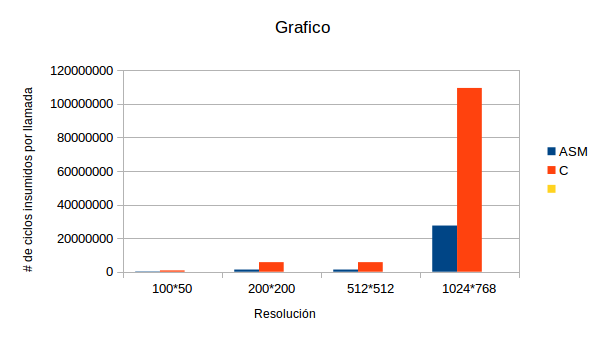
\includegraphics[scale=1]{temperature.png}
 \end{center}
  \vspace*{0.3cm} 
La diferencia principal entre el c\'odigo escrito en lenguaje C y el c\'odigo ASM, es la cantidad de accesos 
a memoria realizados en cada iteraci\'on. Otra diferencia puede verse en la cantidad de bytes que pueden 
ser procesados simultaneamente durante el mismo ciclo. 
Mientras que en C leemos y procesamos un byte por vez, el c\'odigo ASM nos permite acceder y procesar 
16 bytes en simultaneos. De todas maneras, en este caso trabajamos con 12 bytes que es un numero mas \'util 
ya que es m\'ultiplo de 3 (cantidad de bytes por p\'ixel)  y de 4 (cantidad de bytes por cada caracter).
Pudiendo levantar de a 16 bytes en memoria, podr\'ia esperarse que el c\'odigo asm demorase una 
diesiseiava parte de la cantidad de ciclos que demora el c\'odigo en C.
Pero debemos tener en cuenta que en nuestro caso estamos aprovechando solo 15 de los 16 bytes que leemos 
en cada iteraci\'on por lo tanto es más acertado evaluar como si solo leyeramos 15 bytes. 
Adem\'as, hay que tener en cuenta que las instrucciones SSE pueden necesitar más ciclos que las operaciones 
comunes que usamos en el C, eso disminuye un poco la performance en la comparación. 
\vspace*{0.3cm} \vspace*{0.3cm} 
 %Luego de dichas mediciones podemos concluir en que la implementacion en ASM por el uso del 
 %paralelismo con instrucciones sse posee una mejor performance.
 %Además teniendo en cuenta que los accesos a memoria son muy costosos, 
 %el paralelismo hace que se reduzcan estos mismos.
 
 